\documentclass{article}
\usepackage[utf8]{inputenc}
\usepackage[margin={.95in,.75in}]{geometry}
\usepackage{titlesec}
\usepackage{titling}
\usepackage[default,scale=1]{opensans}
\usepackage{graphicx}

\setlength{\parindent}{0em}
\setlength{\parskip}{0.5em}
\renewcommand{\baselinestretch}{1.5}
\pagenumbering{gobble}
\setlength{\hyphenpenalty}{1000}
\setlength{\exhyphenpenalty}{1000}

\author{Ryan Bruno}
\date{\today}

\renewcommand{\maketitle}{
\textbf{\underline{Name:}}
\theauthor

\textbf{\underline{Title:}}
My Mental Map of Shippenburg University's Campus
}

\begin{document}

\maketitle

\textbf{\underline{Analysis}}

\setlength{\parindent}{5ex}
For this assignment, I have created my own mental map of Shippensburg University. I made sure to scale and position the map to include all of the landmarks and paths between them that are significant to me. During my time enrolled at Shippensburg, I have found some areas of campus to be more significant to me as a student while others are rarely visited. For example, buildings such as Henderson Gym and Gilbert I have never been in. Other areas such as Richard Avenue and High Street while technically not on campus are very significant to me as that is where I currently live. Both of these facts are represented in my mental map. 

I have included three landmarks on my mental map. The first of which, Old Main, is the metaphorical center of campus. The large, old building stood on a hill overlooks the entire campus and all its operations. Housing most of the administrators, students may need to visit the building occasionally for academic, financial, or disciplinary reasons. While college is usually all about learning, I had the privilege to incorporate some games into my education; referring to the fact that I was a member of the Football team since my freshman year. As such, a significant proportion of time and therefore my experiences have been in the great Seth Grove Stadium, making it my second landmark. After a day of studying and a practice or game, the best thing to do is head home and relax. My house, being the third landmark, completes the list of significant locations for which deserves the designation of a landmark on my mental map.

I have chosen may nodes for my mental map; the definition of "focal points where people meet or come together" is perfect for the buildings I have chosen. The center of my map is home to the four most important buildings, Franklin, Shippen, DHC/MCT, and the Library, where students come together to explore science, education, technology, and literature. Other buildings, almost located in a ring outside the previous buildings, includes mostly dining halls; the significants of the dining hall to a student include a place to eat, socialize, and sometimes cram study before an exam. The last important node on my mental map in Big Richards, meeting the node definition in two ways. Firstly, a restaurant, similar to a dining hall, attracts many people both student and nonstudent to gather for food but Big Richards is special to me. Friends, teammates, and other colleagues all know where Big Richards is, making it the best place for meeting, using as a refrence, or grabbing a bit to eat. 

A person's perception of a thing will, with their knowledge or not, always change with time; this is especially true with a university campus such as Shippensburg. For example, I lived in Harly Hall hall in my first semester and every one of my classes was located in the adjacent building; Dauphin Humanities Center. If you asked freshman me to draw a mental map of the campus it would be significantly different then the one below and in the future when I revisit campus I will way to myself, "this is different then I remembered."

\begin{figure}[t]
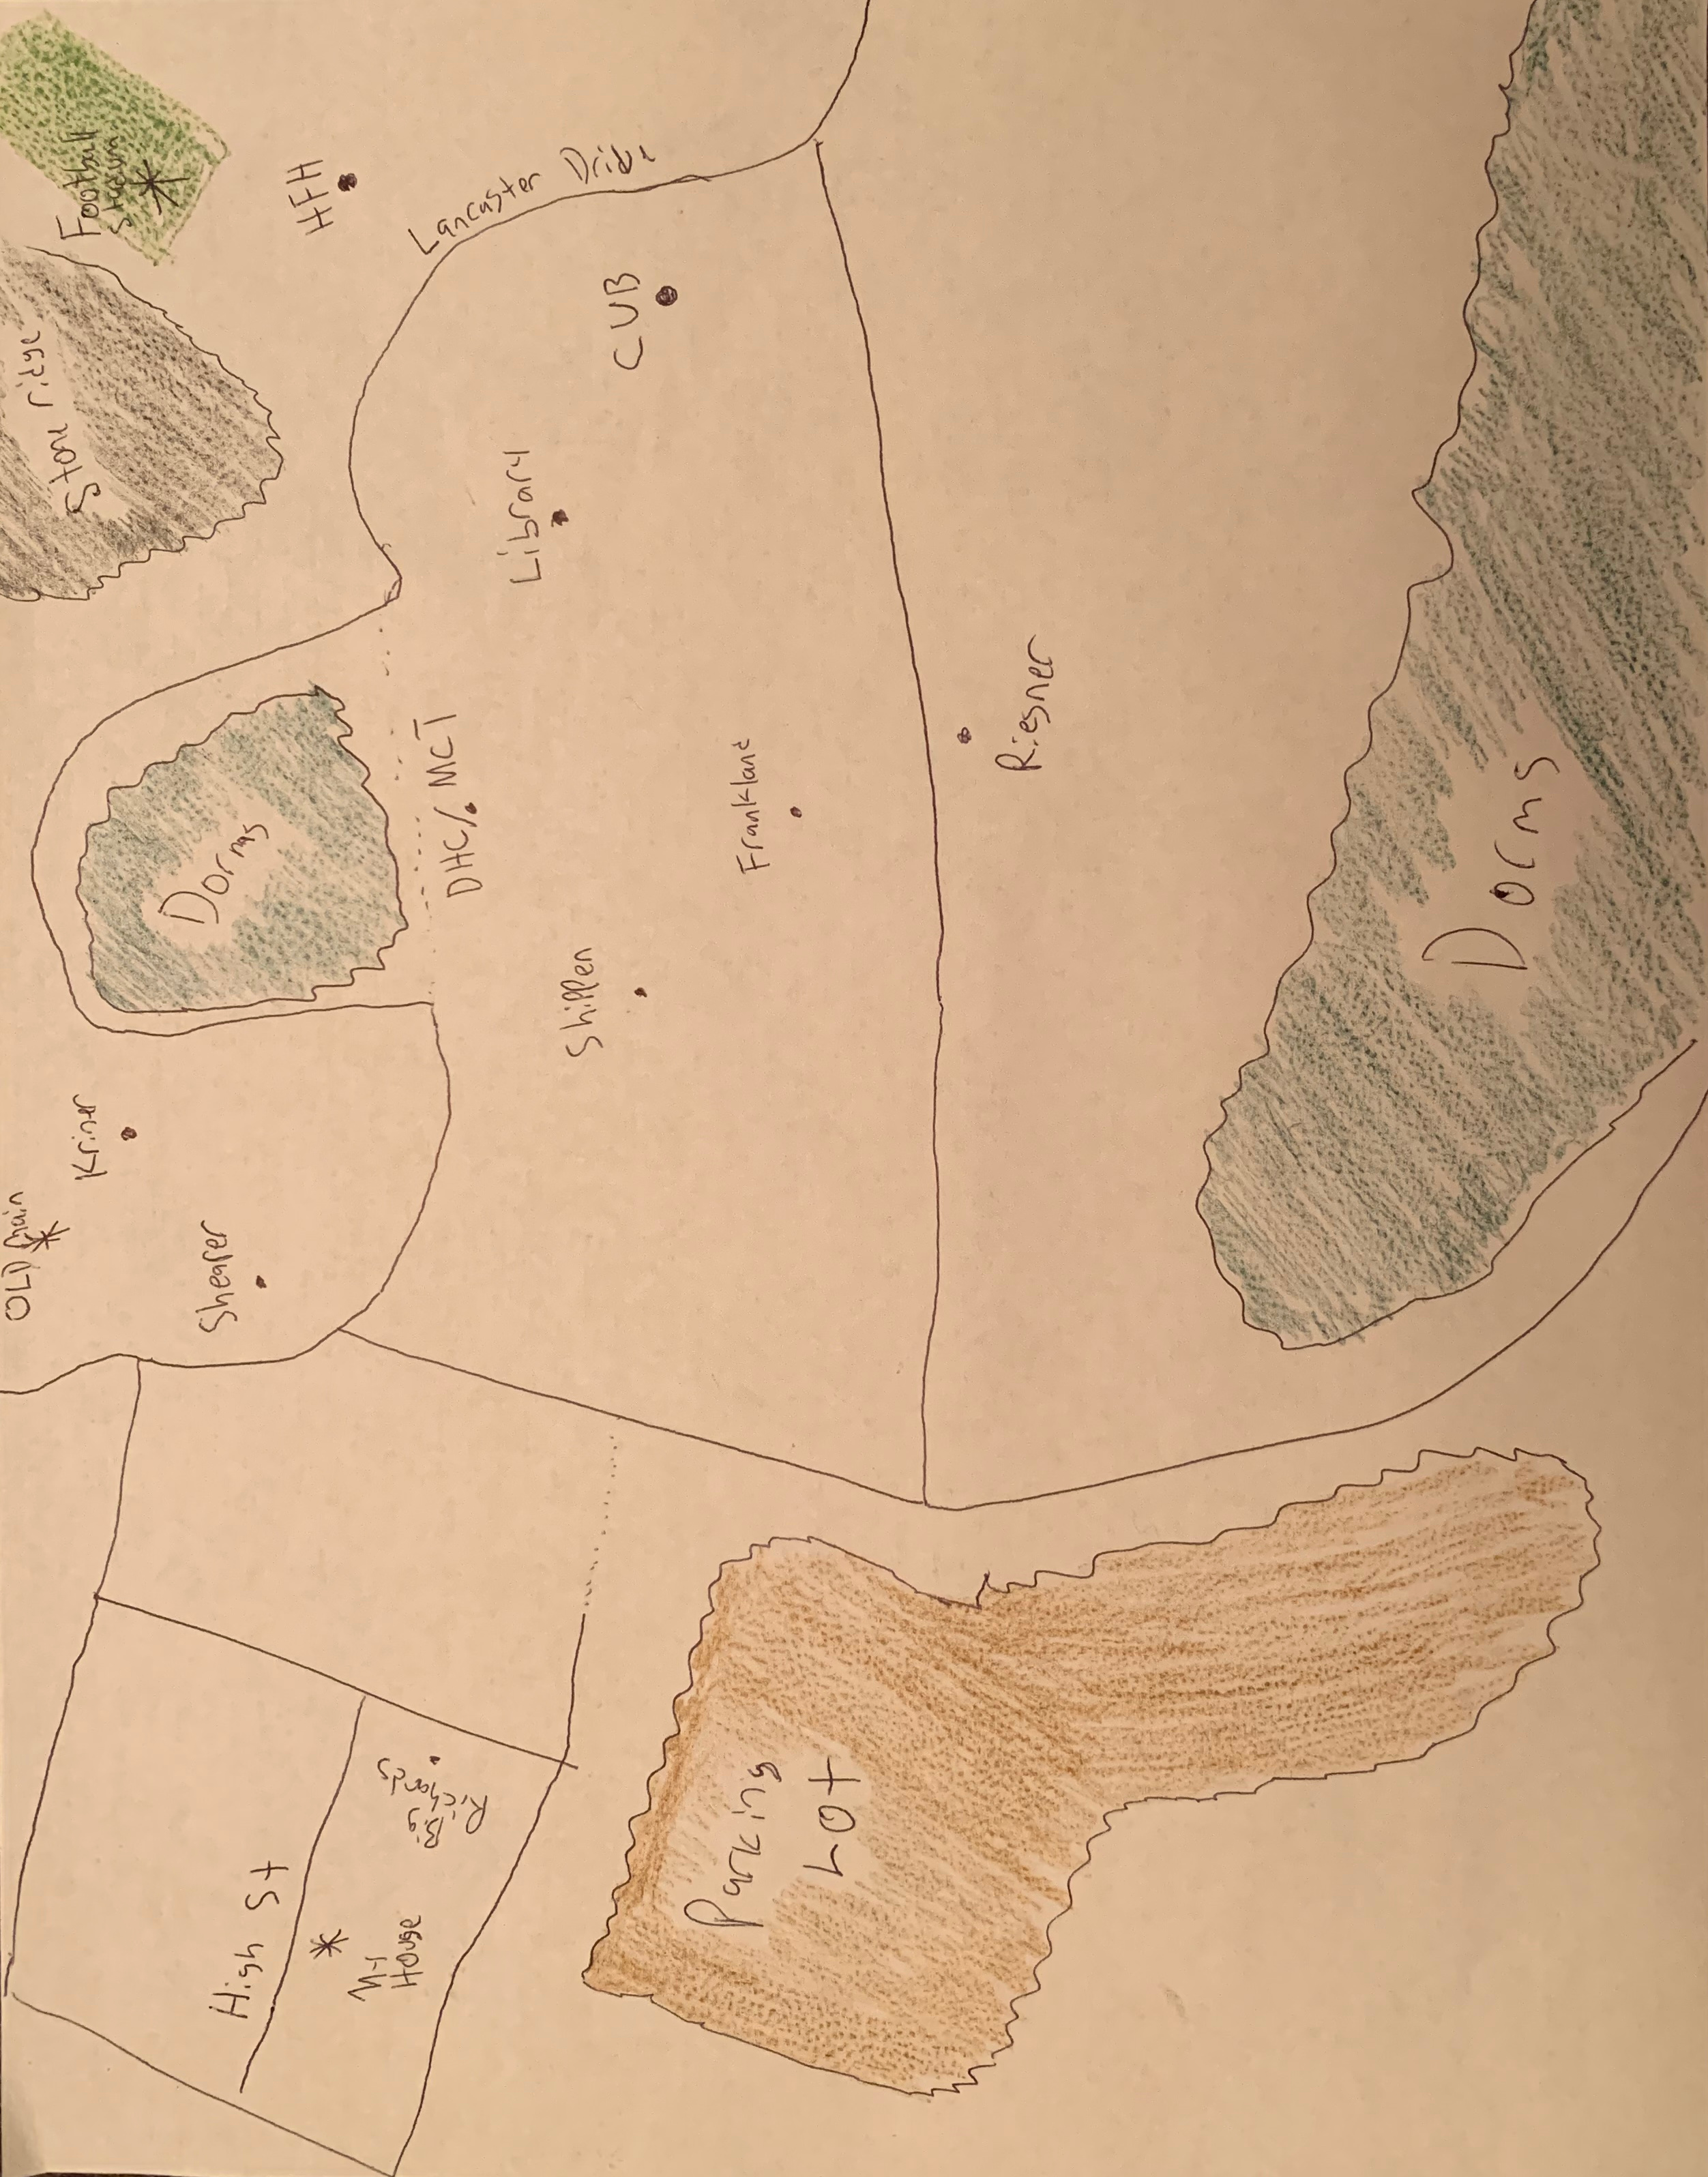
\includegraphics[width=\textwidth]{map}
\end{figure}

\end{document}
